
\section{Ángulo entre elementos de un espacio con producto punto}

Es gracias a la desigualdad de Cauchy-Schwarz
que es posible introducir una de las nociones
más valiosas con las que se cuenta en un espacio
vectorial con producto punto, a saber, la de ángulo entre dos
vectores.

Si $v$ y $w$ son dos elementos no cero de $V$, entonces,
según el teorema \ref{Teo:CauchySchwarz},
\[
-1 \leq \frac{\langle v, w \rangle}{||v|| \cdot ||w||} \leq 1,
\]
luego, puesto que la función coseno es una biyección
del intervalo $[0, \pi]$ al intervalo $[-1,1]$,
tenemos que existe un único elemento 
$\theta \in [0, \pi]$ tal que

\[
cos(\theta)= \frac{\langle v, w \rangle}{||v|| \cdot ||w||};
\]
a tal número $\theta$ se le denomina el 
\textbf{ángulo formado por los vectores $v$ y $w$}.

\begin{marginfigure}
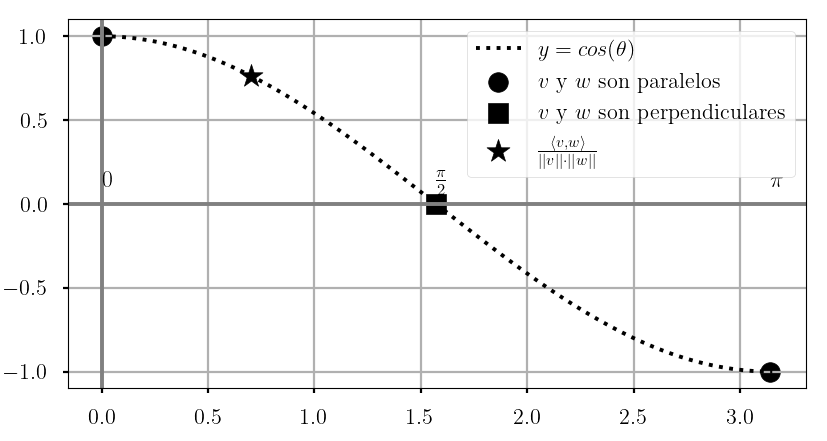
\includegraphics[scale=0.1]{coseno}
\end{marginfigure}

Si alguno de estos dos vectores fuese cero, definimos
el ángulo entre estos como cero. \TODO{Aquí deberías
de poner qué significan los casos extremos. Recuerda
la teoría de Spivak, cálculo en varias variables.}




\section{Definición de ángulo entre un punto y un plano en un espacio euclideo}

Como vimos en \TODO{(ref: justo después de C-S di 
que es gracias a esta desigualdad que puedes definir el
ángulo entre vectores)}, una de las grandes ventajas de tener
definido en un espacio vectorial $V$ un producto punto es
que este conlleva una definición natural de ángulo entre
vectores.

Si además $W$ es un subespacio cerrado de $V$
(lo que, recuerde, siempre ocurre en caso de que
$V$ sea finito dimensional \TODO{ref.}), entonces también
es posible definir el ángulo entre un punto $x \in V$
del espacio y $W$.

\begin{defi} \label{def: angulo punto subespacio}
Sea $(V, \langle \cdot , \cdot \rangle)$ un espacio con 
producto punto. Sean $W \leq V$ un subespacio cerrado de $V$
y $x \in V$. Definimos el \textbf{ángulo entre $x$ y $W$}
como el ángulo que forma 
$x$ con su proyección a $W$, es decir,
\[
\measuredangle (x, W):= \measuredangle(x, \Pi_{W}(x)).
\]
\end{defi}

Una definición alternativa del ángulo entre un punto y un subespacio,
así como una caracterización sencilla del coseno de este,
se dan a continuación.

\begin{prop}
\label{prop: algunos hechos sobre el angulo entre un vector y un subespacio}
Si $V$, $W$ y $x$ son como en la definición 
\ref{def: angulo punto subespacio}, entonces

\begin{itemize}
\item \[
\measuredangle (x, W) = min \{ \measuredangle(x,w) \hspace{0.1cm} :
 \hspace{0.1cm} w \in W \},
\]
y 

\item $cos \left( \measuredangle (x, W) \right) = \frac{|| \Pi_{W}(x) ||}{||x||}$.
\end{itemize}


\end{prop}
\noindent
\textbf{Demostración.}
\begin{itemize}
\item  Sea $w$ un elemento cualquiera de $W$.
Puesto que el ángulo entre dos vectores es
preservado bajo multiplicación por escalares
(c.f. \TODO{debes poner en el apéndice este resultado, 
luego lo citas en el ejemplo}), sin pérdida de generalidad
podemos suponer que 
\begin{equation}
\label{eq1: 9Feb}
||w||= || \Pi_{W}(x)||.
\end{equation}

De la definición del vector $\Pi_{W}(x)$ se sigue que
\[
|| x -\Pi_{W}(x) ||^{2} \leq  || x - w||^{2};
\]
expresando ambos lados de la desigualdad como un producto
punto (c.f. \TODO{referencia}) y aplicando la
bilinealidad del producto punto, llegamos a que
\[
\langle x , x \rangle -2 \langle x, \Pi_{W}(x) \rangle +
\langle \Pi_{W}(x) , \Pi_{W}(x) \rangle \leq 
\langle x , x \rangle  -2 \langle x , w \rangle 
+ \langle w , w \rangle ;
\]
usando \eqref{eq1: 9Feb}, podemos simplificar esta
última desigualdad para llegar a 
\[
\langle x, w \rangle \leq \langle x, \Pi_{W}(x) \rangle,
\]
de donde se sigue, usando nuevamente \eqref{eq1: 9Feb},
que 
\[
cos \left( \measuredangle (x,w) \right) =
\frac{\langle x , w \rangle}{||x||\cdot ||w||} \leq
\frac{\langle x ,  \Pi_{W}(x)  \rangle}{||x||\cdot ||w||} =
cos \left( \measuredangle \left(x, \Pi_{W}(x) \right) \right);
\]
del que la función coseno sea decreciente en el intervalo
$[0, \pi]$ se concluye de esta última desigualdad que
$ \measuredangle \left(x, \Pi_{W}(x) \right) \leq 
\measuredangle (x,w)$.

\item Según el corolario 
\ref{cor: x como suma de proyecciones}, 
$x$ puede expresarse como la suma entre su proyección
a $W$ y su proyección a $W^{\perp}$, luego,
según la definición \ref{def: angulo punto subespacio}
y la linealidad del producto punto, concluimos que

\begin{align*}
cos \left( \measuredangle (x, W) \right) = &
cos \left( \measuredangle (x, \Pi_{W}(x)) \right)  \\
= & 
\frac{\langle x , \Pi_{W}(x) \rangle}{||x|| \cdot || \Pi_{W}(x)||}  \\
= & 
\frac{\langle \Pi_{W}(x)+\Pi_{W\perp}(x) , \Pi_{W}(x) \rangle}{||x|| \cdot || \Pi_{W}(x)||}\\
= & \frac{\langle \Pi_{W}(x) , \Pi_{W}(x) \rangle}{||x|| \cdot || \Pi_{W}(x)||}\\
= & \frac{|| \Pi_{W}(x) ||^{2}}{||x|| \cdot || \Pi_{W}(x)||}\\
= & \frac{|| \Pi_{W}(x) ||}{||x||}.
\end{align*}
\end{itemize}

\QEDB
\vspace{0.2cm}




\TODO{Pon ejemplos gráficos en dimensión 2 y 3.
Creo que en dimensión 2 el ángulo entre $x$ y un vector
de $W$ es siempre el mismo.}


\subsection{Caso particular en el que el subespacio en cuestión es un plano}
\label{ap: Caso particular en el que el subespacio en cuestión es un plano}

Para terminar este apartado, vamos a
agregar unos resultados que serán usados en la teoría
\TODO{mejora descripción.}


La situación es la siguiente: $V$ es un $\IR-$espacio
de Hilbert, $u$ y $v$ son elementos de $V$,
unitarios y linealmente
independientes entre sí. El espacio que ellos generan
es pues un plano, digamos,


\[
P= span \{ u, v \}
\]

Dado $x \in V$ unitario, nos gustaría dar una medida
de la cercanía de $x$ con el espacio $P$; si tomamos
al coseno del ángulo como una tal medida, según la proposición
\ref{prop: algunos hechos sobre el angulo entre un vector y un subespacio},

\begin{equation}
\label{eq0: 19Marzo}
cos \left( \measuredangle (x, P) \right) = || \Pi_{P}(x) ||;
\end{equation}
para lograr expresar el lado derecho de la igualdad en términos
sólo de $u$, $v$ y $x$ (que son los elementos básicos de
nuestra discusión), conviene primero considerar una base
ortonormal del espacio $P$.


\begin{obs}
Si $u, v \in V$ son unitarios y linealmente independientes, y $P$
es el plano que generan, entonces
$\{ u, z \}$, donde

\begin{equation}
\label{eq2: 19Marzo}
z:= \frac{v- \langle u, v \rangle u}{||v- \langle u, v \rangle u||}
\end{equation}
es una BON de $P$
\end{obs}
\noindent
\textbf{Demostración.}
Basta aplicar el teorema de Gram-Schmidt 
\ref{Teo:Gram-Schmidt}.
\QEDB
\vspace{0.2cm}

Teniendo una BON de $P$ se obtiene, via la prop.
y la expresión \eqref{eq0: 19Marzo},
\TODO{ref; debes de poner la discusión de BON mucho antes!!}
se obtiene una expresión de la proyección de $x$ al plano $P$ en función
de $x$, $u$ y $z$;

\begin{equation}
\label{eq1: 19Marzo}
\Pi_{P}(x)= \langle x, u \rangle u + \langle x, z \rangle z;
\end{equation}

puesto que, según la definición \eqref{eq2: 19Marzo} de 
$z$ este vector es función de $u$ y $v$, fácilmente se
deriva una expresión de $\Pi_{P}(x)$ (y, por lo tanto, una
medida de la cercanía de $x$ al plano $P$) en función sólo
de $x$, $u$ y $v$.

	\begin{prop}
	\label{prop: formulas 20Marzo}
	si $x, u, v \in V$ y $P \subseteq V$ son como en la discusión anterior
	(\TODO{pon aquí las hipótesis!}),
	entonces 

		\begin{equation}
		\label{eq3: 19Marzo}
		\Pi_{P}(x)= \frac{\langle x, u \rangle -\langle u, v \rangle \langle x, v \rangle }{1-\langle u, v \rangle^{2}} u + \frac{\langle x, v \rangle -\langle u, v \rangle \langle x, u \rangle }{1-\langle u, v \rangle^{2}} v
		\end{equation}
	y 
		\begin{equation}
		\label{eq3: 19Marzo}
		  || \Pi_{P}(x) ||^{2}=
		  \frac{1}{1- \langle u, v \rangle^{2}} \left(  
	       \langle x, u \rangle^{2} +  \langle x, v \rangle^{2}	
	       -2  \langle x, u \rangle^{2} \langle x, v \rangle^{2} \langle u, v \rangle^{2}	  
		  \right).
		\end{equation}
 
	\end{prop}

